\documentclass{beamer}
%
% Choose how your presentation looks.
%
% For more themes, color themes and font themes, see:
% http://deic.uab.es/~iblanes/beamer_gallery/index_by_theme.html
%
\mode<presentation>
{
  \usetheme{Madrid}      % or try Darmstadt, Madrid, Warsaw, ...
  \usecolortheme{default} % or try albatross, beaver, crane, ...
  \usefonttheme{default}  % or try serif, structurebold, ...
  \setbeamertemplate{navigation symbols}{}
  \setbeamertemplate{caption}[numbered]
}

\usepackage[english]{babel}
\usepackage[utf8x]{inputenc}
\usepackage{multirow}
\usepackage{booktabs}
\usepackage{graphicx}
\usepackage{tikz,pgfplots}
\usepackage{caption}
\usepackage{appendixnumberbeamer}
\usepackage{tikz}
\makeatletter

\usepackage{bbm} %indicator fct
\usepackage{natbib} %Literature
%\usepackage{apacite}

\pgfplotsset{compat=1.14}


% settings for tree
  \tikzset{
	invisible/.style={opacity=0},
	visible on/.style={alt={#1{}{invisible}}},
	alt/.code args={<#1>#2#3}{%
		\alt<#1>{\pgfkeysalso{#2}}{\pgfkeysalso{#3}} % \pgfkeysalso doesn't change the path
	},
}


\title[Bagging Regression Trees]{Bagging Regression Trees}
\author[Kraft, Werner, Zeimentz]{Robin Kraft, Tobias Felix Werner and David Zeimentz}
\institute[Uni. Bonn]{University of Bonn}
\date{17.01.2018}

\begin{document}

\begin{frame}
  \titlepage
\end{frame}

%%%%%%%%%Introduction%%%%%%%%%%%%%%%%%%%%%%%%%%%%%%%%%%%%%%%%%%%%%%%%
%%%%%%%%%

%\begin{frame}{Introduction}
%\begin{itemize}
%\item \textbf{Application:} Prediction
%\item \textbf{Problem}: Inherent Bias-Variance Trade-off
%\item \textbf{Example:} Regression Trees
%\begin{itemize}
%\item low Bias\\
%\item high Variance\\
%$\Rightarrow$ \textbf{poor prediction accuracy}
%\end{itemize}
%\item \textbf{Aim}: Construct an algorithm that can improve the prediction performance (MSE) by reducing the variance while not increasing the bias too much.

%\end{itemize}
%\end{frame}

%%IntroVorschlagROBIN%%%%%%%%%%%%%%%%%%%%%%%%%%%%%%%%%%%%%%%%%%%%%%%

%\begin{frame}{Introduction - Vorschlag Robin}
%\begin{itemize}
%\item \textbf{Recall Multivariate Linear Regression Model:}
%$$
%Y = X\beta  + \gamma X X^{T} + \epsilon,
%Formel passt noch nicht ganz von den Dimensionen
%$$

%Model real-valued vector $Y \in \mathbb{R}^{n}$ as a linear function of real-valued covariate matrix $X \in \mathbb{R}^{n x p}$ and noise $\epsilon \in \mathbb{R}^{n}$
%where $Y \in  \mathbb{R}^{n}$ is real-valued response, \\
%$X \in \mathbb{R}^{n x p}$ is the covariate matrix and \\
%$\epsilon \in \mathbb{R}^{n}$ is the error term
%\item \textbf{Global model:} Single prediction formula holds over entire data space

%\item \textbf{Problem:} not possible to model many features that interact in complicated, nonlinear ways\\
%$\Rightarrow$ Regression Trees
%\end{itemize}
%\end{frame}

%\begin{frame}{Introduction - Vorschlag Robin}
%\begin{itemize}
%\item \textbf{Another Problem:} Trees tend to overfit the data $\rightarrow$ predictors have high variance


%\item \textbf{Idea:} Average over multiple trees constructed via bootstrapping \\

%\item \textbf{Aim:} Reduce the variance while not increasing the bias „too much“\\
%$\Rightarrow$ Bagging (Bootstrap Aggregation)

%\item Economic Relevance: ...?
%\end{itemize}


%\end{frame}


%%%Intro Vorschlag Tobi%%%%%


\begin{frame}{Introduction}
\begin{itemize}
\item \textbf{Goal}: Prediction of a real-valued response variable $Y\in R^{n}$ based on covariate matrix $X\in R^{n\:x\:p}$
\item \textbf{Problem}: Common prediction methods inherent a Bias-Variance trade-off
% * <saibotwerner@gmail.com> 2018-01-13T14:24:47.216Z:
%
% Hier würde ich dann den Trade-off erklären. Das kann man ja sogar an einem linearen Model machen. Mehr interactions -> Lower Bias but higher Variance etc
%
%
% ^.
\item \textbf{Our Objective}: Introduce to you the Bagging algorithm that bypasses this trade-off for certain predictors
% * <saibotwerner@gmail.com> 2018-01-13T14:34:08.470Z:
%
% "It turns out that we can bypass this trade-off for a certain type of predictors. Namely those that have a low bias and a high Variance.
%
% ^.
\end{itemize}
\end{frame}

\begin{frame}{Introduction}
\begin{itemize}
\item Consider Regression Trees as an explanatory predictor
%point out that we will explain Regression Trees further over the course of this presentation
	\begin{itemize}
	\item Low Bias %Say verbally that they are suited to fit complex nonlinear data with a low bias and why
    \item High variance % They exhibit this high variance as they tend to overfit the data. Therefore Regression Trees are usually not competitively viable for prediction purposes relative to other predictors and algorithms

	\end{itemize}
\item Bagging improves the prediction accuracy for Regression Trees by reducing its Variance
\item Bagging used on Regression Trees becomes a powerful prediction tool
% Widely used in industries and academia for prediction purposes. With slight further modifications this combination is known under the name Random Forest, which is the 'Go-To' Machine Learning Tool for lots of different application purposes.

\end{itemize}
% * <saibotwerner@gmail.com> 2018-01-13T15:12:16.799Z:
%
% Bagging, which we will introduce within this presentation, can reduce the variance while leaving the Bias of the specific predictor almost unaffected.
% There by we can greatly reduce the variance of our predictor and thus substantially increase the prediction results of predictors.
%
%
% ^.
% * <saibotwerner@gmail.com> 2018-01-13T15:31:44.295Z:
%
% - We show here that bagging can drastically reduce the Variance of Regression Trees
% - We will explain you Bagging
% - Give you theoretical insight why Bagging works specifically well with Trees
% - For this purpose we will begin our presentation by introducing you to regression Tree and explain you some properties of this prediction method
%
% ^.
\end{frame}


%%%%%TableofContents%%%%%%%%%%%%%%%%%%%%%%%%%%%%%%%%%%%%%%%%%%%%%%%%
\begin{frame}{Outline}
  \tableofcontents
\end{frame}


%%%%%%%DavidPart%%%%%%%%%%%%%%%%%%%%%%%%%%%%%%%%%%%%%%%%%%%%%%%%%%%%%%

%%%%%%%%%
%\section{Stability}
%\begin{frame}{Stability of a Predictor}

%\textbf{Data:} $L_{i}=(Y_{i}, X_{i})$ i.i.d., where $Y_{i}$ real-valued response, $X_{i}$ $p$-dimensional explanatory variable

%\begin{definition}[Stability of a predictor (\cite{Buhlmann2002})] \label{stability}
%A statistic $\hat{\theta}_{n}(x) = h_{n}(L_{1},\dots, L_{n})(x)$ is called stable at $x$ if $\hat{\theta}_{n}(x) = \theta(x) + o_{p}(1) \quad (n \rightarrow \infty)$ for some fixed value $\theta(x)$.
%\end{definition}

%\end{frame}

%%%%%%%%%%
\section{Regression Trees}
\begin{frame}{Regression Trees}{Prediction using Regression Trees}
\begin{itemize}
\item Prediction of an outcome $Y$ using three explanatory variables $\textbf{X}=(X_1,X_2,X_3) \in [0,1]^3$\\
\item Example: $\textbf{X}^1=(0.4,0.4,0.9)$
\end{itemize}

\begin{figure}
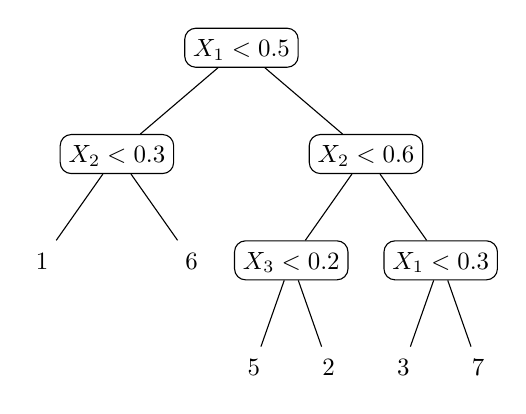
\begin{tikzpicture}[
scale = 0.9,
every node/.style={transform shape},
baseline,
level distance=15mm,
text depth=.1em,
text height=.8em,
level 1/.style={sibling distance=10em},
level 2/.style={sibling distance=6em},
level 3/.style={sibling distance=3em}]


	\node [rounded corners, draw] {$X_1 < 0.5$}
		child {node [rounded corners, draw] {$X_2 < 0.3$}
			child {node {$1$}}
			child {node {$6$}}
		}
		child {node [rounded corners, draw] {$X_2 < 0.6$}
			child {node [rounded corners, draw] {$X_3<0.2$}
				child {node {$5$}}
				child {node {$2$}}
			}
			child {node [rounded corners, draw] {$X_1<0.3$}
				child {node {$3$}}
				child {node {$7$}}
			}
	};



\end{tikzpicture}
\caption{Illustration of a Regression Tree}
\end{figure}

\end{frame}

%%%%%%%%%%%%%%%%%%%%%%%%%%%%%%%

\begin{frame}{Regression Trees}{Prediction using Regression Trees}
\begin{itemize}
\item Prediction of an outcome $Y$ using three explanatory variables $\textbf{X}=(X_1,X_2,X_3) \in [0,1]^3$\\
\item Example: $\textbf{X}^1=(0.4,0.4,0.9)$
\end{itemize}

\begin{figure}
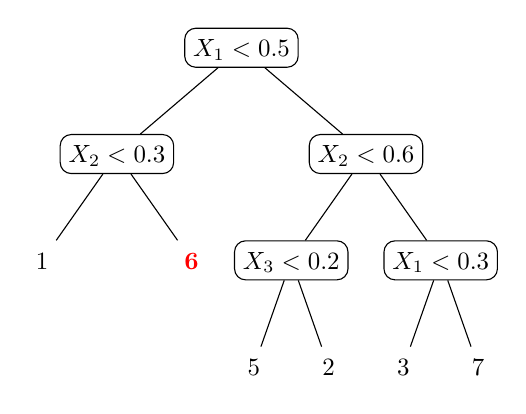
\begin{tikzpicture}[
scale = 0.9,
every node/.style={transform shape},
baseline,
level distance=15mm,
text depth=.1em,
text height=.8em,
level 1/.style={sibling distance=10em},
level 2/.style={sibling distance=6em},
level 3/.style={sibling distance=3em}]


	\node [rounded corners, draw] {$X_1 < 0.5$}
		child {node [rounded corners, draw] {$X_2 < 0.3$}
			child {node {$1$}}
			child {node [red ]{$\textbf{6}$}}
		}
		child {node [rounded corners, draw] {$X_2 < 0.6$}
			child {node [rounded corners, draw] {$X_3<0.2$}
				child {node {$5$}}
				child {node {$2$}}
			}
			child {node [rounded corners, draw] {$X_1<0.3$}
				child {node {$3$}}
				child {node {$7$}}
			}
	};



\end{tikzpicture}
\caption{Illustration of a Regression Tree}
\end{figure}

\end{frame}

%%%%%%%%%%%%%%%%%%%%%%%%%%%%%%%


\begin{frame}{Regression Trees}{CART}

\begin{columns}[T]
    \begin{column}{5cm}
    \begin{figure}
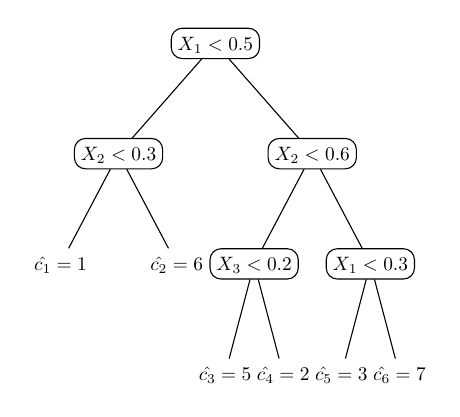
\begin{tikzpicture}[
scale = 0.7,
every node/.style={transform shape},
baseline,
level distance=20mm,
text depth=.1em,
text height=.8em,
level 1/.style={sibling distance=10em},
level 2/.style={sibling distance=6em},
level 3/.style={sibling distance=3em}]


	\node [rounded corners, draw] {$X_1 < 0.5$}
		child {node [rounded corners, draw] {$X_2 < 0.3$}
			child {node {$\hat{c_1}=1$}}
			child {node {$\hat{c_2}=6$}}
		}
		child {node [rounded corners, draw] {$X_2 < 0.6$}
			child {node [rounded corners, draw] {$X_3<0.2$}
				child {node {$\hat{c_3}=5$}}
				child {node {$\hat{c_4}=2$}}
			}
			child {node [rounded corners, draw] {$X_1<0.3$}
				child {node {$\hat{c_5}=3$}}
				child {node {$\hat{c_6}=7$}}
			}
	};

\end{tikzpicture}
\caption{Illustration of a Regression Tree}
\end{figure}

    \end{column}


    \begin{column}{5cm}
		\textbf{CART Algorithm:}
        \begin{enumerate}
        	\item <1-> Consider all observations
			\item <2-> Choose split variable and split point minimizing RSS in 					  subsets
			\item <3-> Repeat procedure for the resulting subsets ...
			\item <4-> ... until stopping rule is satisfied
            \item <5-> Fit a constant for each terminal node
		\end{enumerate}
	\end{column}


\end{columns}

\end{frame}


%%%%%%%%%%%%%%%%%%%%%%%%%%%%%%%%%%%%%%%%%%%%%%%%%%%%%%%%%%%%%%%%%%%%%%%%%%%%%%

\begin{frame}{Regression Trees}{Predictor}
For a given tree with $M$ terminal nodes, denoted as $R_m $ $(m= 1, \dots, M)$, the tree predictor is given by

$$\hat{\theta}_{n}(x)=\sum\limits_{m=1}^{M}\hat{c}_m\mathbbm{1}_{[x\in R_m]}$$

\ \\
where $\hat{c}_m$ denotes the outcome average of observations within each terminal node

\ \\

\end{frame}



%%%%%%%%%%%%%%%%%%%%%%%%%%%%%%%%%%%%%%%%%%%%%%%%%%%%%%%%%%%%%%%%%%%%%%%%%%%%%

\begin{frame}{Regression Trees}{Bias, Variance and Instability}

\textbf{Instability}: A small perturbation in the data set leads to significant changes in the predictor

\begin{columns}[T]
    \begin{column}{5cm}
    \begin{figure}
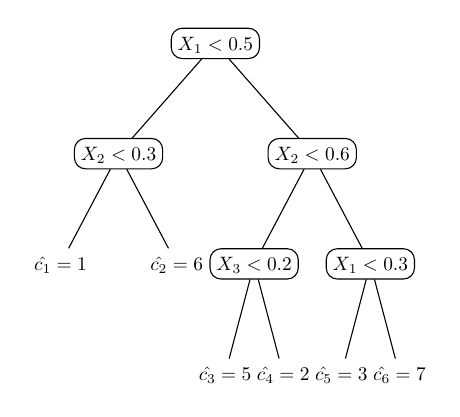
\begin{tikzpicture}[
scale = 0.7,
every node/.style={transform shape},
baseline,
level distance=20mm,
text depth=.1em,
text height=.8em,
level 1/.style={sibling distance=10em},
level 2/.style={sibling distance=6em},
level 3/.style={sibling distance=3em}]


	\node [rounded corners, draw] {$X_1 < 0.5$}
		child {node [rounded corners, draw] {$X_2 < 0.3$}
			child {node {$\hat{c_1}=1$}}
			child {node {$\hat{c_2}=6$}}
		}
		child {node [rounded corners, draw] {$X_2 < 0.6$}
			child {node [rounded corners, draw] {$X_3<0.2$}
				child {node {$\hat{c_3}=5$}}
				child {node {$\hat{c_4}=2$}}
			}
			child {node [rounded corners, draw] {$X_1<0.3$}
				child {node {$\hat{c_5}=3$}}
				child {node {$\hat{c_6}=7$}}
			}
	};

\end{tikzpicture}
\caption{Regression Tree using \textbf{initial} Data}
\end{figure}

    \end{column}


    \begin{column}{5cm}
\begin{figure}
		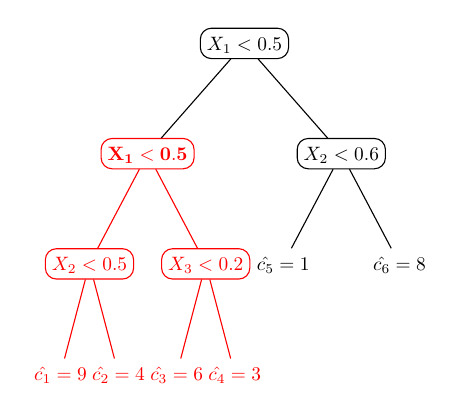
\begin{tikzpicture}[
		scale = 0.7,
		every node/.style={transform shape},
		baseline,
		level distance=20mm,
		text depth=.1em,
		text height=.8em,
		level 1/.style={sibling distance=10em},
		level 2/.style={sibling distance=6em},
		level 3/.style={sibling distance=3em}]


		\node [rounded corners, draw] {$X_1 < 0.5$}
		child {node [red, rounded corners, draw] {$\mathbf{X_1 < 0.5}$}
			child [red] {node [rounded corners, draw] {$X_2<0.5$}
				child {node {$\hat{c_1}=9$}}
				child {node {$\hat{c_2}=4$}}
				}
			child [red] {node [rounded corners, draw] {$X_3<0.2$}
				child {node {$\hat{c_3}=6$}}
				child {node {$\hat{c_4}=3$}}
				}
		}
		child {node [rounded corners, draw] {$X_2 < 0.6$}
			child {node {$\hat{c_5} = 1$}}
			child {node {$\hat{c_6} = 8$}}
		};

		\end{tikzpicture}
        \caption{Regression Tree using \textbf{perturbed} Data}
	\end{figure}
	\end{column}


\end{columns}

\end{frame}

%%%%%%%%%%%%%%%%%%%%%%%%%%%%%%%%%%%%%%%%%%%%%%%%%%%%%%%%%%%%%%%%%%%%%%%%%

%%%%%%%RobinPart%%%%%%%%%%%%%%%%%%%%%%%%%%%%%%%%%%%%%%%%%%%%%%%%%%%%%
\section{Bagging}
\begin{frame}{Bagging (Bootstrap Aggregation) (\cite{Breiman1996})}{Algorithm}
\begin{definition}[Bagging Algorithm (\cite{Buhlmann2002})] \label{bagging}
	\begin{enumerate}

	\item Construct a bootstrap sample $L_{i}^{*} = (Y_{i}^{*}, X_{i}^{*}) \quad (i = 1, \dots , n)$ (with replacement) according to the empirical distribution of the pairs $L_{i} = (Y_{i}, X_{i}) \: i.i.d. \quad (i = 	1, \dots , n).$
	\item Compute the bootstrapped predictor $\hat{\theta}_{n}^{*}(x)$ by the plug-in principle; that is, $\hat{\theta}_{n}^{*}(x) = h_{n}(L_{1}^{*}, \dots, L_{n}^{*})(x)$, where $\hat{\theta}_{n}(x) = h_{n}(L_{1},\dots, L_{n})(x)$.
	\item The bagged predictor is $\hat{\theta}_{n;B}(x) = E^{*} [\hat{\theta}_{n}^{*}(x)]$

	\end{enumerate}
\end{definition}

\textbf{Claim:} Bagging reduces the variance of unstable predictors

%\begin{definition}[Stability of a predictor (\cite{Buhlmann2002})] \label{stability}
%A statistic $\hat{\theta}_{n}(x) = h_{n}(L_{1},\dots, L_{n})(x)$ is called stable at $x$ if $\hat{\theta_{n}}(x) = \theta(x) + o_{p}(1) \quad (n \rightarrow \infty)$ for some fixed value $\theta(x)$.
%\end{definition}

\end{frame}

\begin{frame}{Bagging}{Algorithm}
\begin{figure}
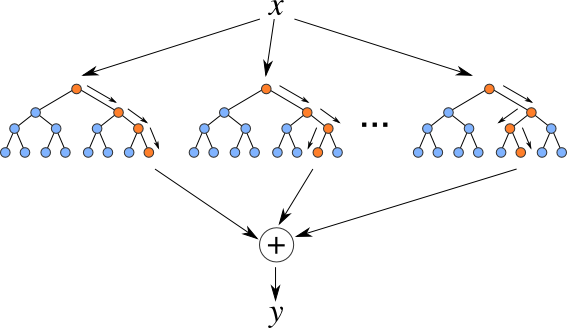
\includegraphics[scale=0.4]{external_figures/baggedtree.png}
\caption{Exemplary prediction procedure after the bagging predictor has been fitted to the data. X being an input matrix of explanatory variables and Y the vector of the according predicted values.}

\end{figure}

\end{frame}




 %%%%%%%%%%

\begin{frame}{Introductory example (\cite{Buhlmann2002})}
\begin{itemize}
\item Let $Y_{1}, Y_{2}, \dots, Y_{n}$ be i.i.d random variables with $\mu = E[Y_{1}]$ and $\sigma^{2} = Var(Y_{1})$.
\item Consider first unbagged predictor,

\begin{equation}\label{unbagged}
\hat{\theta}_{n}(x) = \mathbbm{1}_{[\bar{Y}_{n} \leq x]},\quad x\in  \mathbb{R},
\end{equation}

where $\bar{Y}_{n} = \frac{1}{n}\sum_{i=1}^{n}Y_{i}.$\\

\item \textbf{Note:} Predictor stabilizes (for $n \rightarrow \infty,$ $Var(\hat{\theta}_{n}(x)) \rightarrow 0$)

\end{itemize}

%\textbf{Stability:}
%\begin{itemize}
%\item By (Weak) law of large numbers, $\bar{Y}_{n}\xrightarrow{p} \mu$
%\item By Definition \ref{stability}, $\mathbbm{1}_{[\bar{Y}_{n} \leq x]} = \mathbbm{1}_{[\mu \leq x]} + o_{p}(1)$
%\item $P(Var(\hat{\theta}_{n}(x))>0) \rightarrow 0$
%\end{itemize}
%\\
%The considered predictor converges to a fixed target $\theta(x) = \mathbbm{1}_{[\mu \leq x]}$ and hence stabilizes according to Definition \ref{stability} as $n$ increases.\\
%Moreover, $P(Var(\hat{\theta}_{n}(x))>0) \rightarrow 0.$
\end{frame}

\begin{frame}{Introductory example (\cite{Buhlmann2002})}{Local instability of the predictor}
\begin{itemize}
\item Dynamic threshold:
\begin{equation}\label{12region}
 x = x_{n}(c)= \mu + c\sigma n^{-1/2}
\end{equation}

%Justification via (ordinary) CLT:

%\begin{equation}\label{clt}
%n^{1/2}(\bar{Y}_{n} - \mu ) \xrightarrow{D} \mathcal{N}(0,\,\sigma^{2}),
%\end{equation}

\item Plugging (\ref{12region}) into (\ref{unbagged}) and applying CLT, one yields
$$\hat{\theta}_{n}(x) \xrightarrow{D} \mathbbm{1}_{[Z \leq c]}, \quad Z= n^{1/2} \frac{(\bar{Y}_{n} - \mu )}{\sigma} \sim \mathcal{N}(0,1)$$

\item \textbf{Note:} Unstable Predictor (for $n \rightarrow \infty,$ $Var(\hat{\theta}_{n}(x_{n}(c))) > 0$)
%Moments of the unbagged predictor:
%$$E[\hat{\theta}_{n}(x)] \rightarrow P[Z \leq c] = \Phi(c)\quad (n \rightarrow \infty)$$
%$$Var[\hat{\theta}_{n}(x)] \rightarrow \Phi(c)(1-\Phi(c)) \quad(n \rightarrow \infty)$$
\end{itemize}
\end{frame}

\begin{frame}{Introductory example (\cite{Buhlmann2002})}{Bagged Predictor}
\begin{itemize}
\item For a bagged predictor as in Definition \ref{bagging}, it holds that

\begin{equation}
\begin{split}
\hat{\theta}_{n;B}(x_{n}(c)) & =E^{*}[\mathbbm{1}_{[\bar{Y}_{n}^{*} \leq x_{n}(c)]}]\\
& \xrightarrow{D} \Phi(c-Z),\quad Z \sim \mathcal{N}(0,1)
\end{split}
\end{equation}

\item \textbf{Crucial Assumption:} Bootstrap consistency of $\bar{Y}_{n}$
\end{itemize}
\end{frame}

%\begin{frame}{Case $c=0$}{Introductory example (\cite{Buhlmann2002})}
%$Var[\hat{\theta}_{n}(x_{n}(0))]$ is the highest and the unbagged predictor is the most unstable.

%$$\hat{\theta}_{n;B}(x_{n}(0))\xrightarrow{D} \Phi(-Z) = U, \quad U \sim Uniform([0,1]),$$
%where the last equality holds due to the uniform integral transform.
%\end{frame}


%\begin{frame}
%\textbf{Moments of the bagged predictor:}
%$$E[\hat{\theta}_{n;B}(x_{n}(0))] \rightarrow E[U]=1/2 \quad (n \rightarrow \infty)$$
%$$Var[\hat{\theta}_{n;B}(x_{n}(0))] \rightarrow Var[U]=1/12 \quad (n \rightarrow \infty)$$

%\textbf{Moments of the unbagged predictor:}
%$$E[\hat{\theta}_{n}(x_{n}(0))] \rightarrow \Phi(0)=1/2 \quad (n \rightarrow \infty)$$
%$$Var[\hat{\theta}_{n}(x_{n}(0))] \rightarrow 1/2(1-1/2) = 1/4 \quad (n \rightarrow \infty)$$

%$\Rightarrow$ Bagging reduces the variance by a factor of 3

%\end{frame}

\begin{frame}{Introductory example (\cite{Buhlmann2002})}{Bias-Variance-Tradeoff of the indicator predictor from (\ref{unbagged})}
\begin{center}
\begin{figure}
\includegraphics[scale=0.45]{../../out/figures/theory_part_simulation/plot_toy_example.pdf}
\caption{Variance, squared bias and asymptotic mean-squared error for the predictor in (\ref{unbagged}) and a bagged version as a function of $c$.}
\end{figure}
\end{center}
\end{frame}



\section{Subagging}
\begin{frame}{(Su)bagging stumps}{Failure of bootstrap consistency}
\begin{itemize}
\item Focus on stumps, for extension to full regression trees consult \cite{Buhlmann2002}
\item For stump-predictors (one-split, two terminal nodes), \cite{Buhlmann2002} (Theorem 3.1.) show that
\begin{itemize}
	\item{the convergence rate is $n^{-1/3}$}
    \item{the distribution is non-normal}
\end{itemize}
$\Rightarrow$ Bootstrap is not consistent\\

\item \textbf{Idea:} Generate subsamples by drawing without replacement from the data\\
%Resampling over smaller subsets of the data without replacement
$\Rightarrow$ Subsample Aggregation (Subagging)\
\end{itemize}

\end{frame}



\begin{frame}{Subagging stumps}{Some Remarks}
For $m = [an]$ with $0 < a < 1$,
\begin{itemize}
\item derive upper bounds for the variance and MSE of the subagged stump predictor under very mild assumptions
\item if the dynamic threshold is chosen suitably then
$$
limsup_{n \rightarrow \infty}MSE[\hat{\theta}_{n;SB(m)}(x_{n}(c))] < MSE[\hat{\theta}_{n}(x_{n}(c))],
$$
where $\hat{\theta}_{n;SB(m)}(\cdot)$ is a subagged predictor.

%\item \textbf{Remark:} For $x$ chosen to be in a suitable interval around $\mu$, it follows that
%$$
%limsup_{n \rightarrow \infty}\frac{E[(\hat{\theta}_{n;SB(m)}(x_{n}(c))-E[\hat{\theta}_{n}(x_{n}(c))])^2]}{E[(\hat{\theta}_{n}(x_{n}(c))-E[\hat{\theta}_{n}(x_{n}(c))])^2]} < 1,
%$$
%where the subsample size is given by $m = [an]$ with $0 < a < 1$ and $\hat{\theta}_{n;SB(m)}(.)$ is a subagged predictor.

%\item The discussion carries over to stump predictors ($\rightarrow$ details in the seminar paper)
\end{itemize}

\end{frame}



%%%%%%%TobiPart%%%%%%%%%%%%%%%%%%%%%%%%%%%%%%%%%%%%%%%%%%%%%%%%%%%%%%%
\section{Simulation}


\begin{frame}{Simulation}{Model and Setup}
The Data $\{y_{i},X_{i} \}_{i=1}^{n}$ has been generated according to $$y_{i} = f(X_{i}) + \epsilon_{i}$$
$$\text{with }\epsilon_{i} \sim N(0,1) \text{ and } X_{i} \sim Uniform^{10}([0,1])$$
\begin{itemize}
\item Two regression functions $f(X)$:
\begin{itemize}
\item Friedman \#1 Model: $f(X) = 10 \sin(\pi x_{1} x_{2}) + 20(x_{3} - \frac{1}{2})^{2} + 10 x_{4} + 5 x_{5} $
\item Linear Model: \hspace{9mm} $f(X) = \sum_{j=1}^{5} j \cdot x_{j} $
\end{itemize}
\item $n=500$, number of bootstrap iterations $B=50$ and 100 simulation runs
\end{itemize}


\end{frame}


\begin{frame}{Simulation}{The Effect of Bagging}
\begin{table}
\resizebox{11cm}{!}{
\begin{tabular}{ l l c c c c}
\toprule
\textbf{Model} & \textbf{Method} & \textbf{MSE} &\textbf{Variance} & \textbf{Bias$^{2}$} & \textbf{Relative Error}\tabularnewline
\toprule
\multirow{2}{*}{Friedman \# 1}
& Tree & 9.94 & 6.58 & \textcolor{red}{\textbf{2.36}} & \multirow{2}{*}{0.53}\tabularnewline
& Bagging & \textcolor{red}{\textbf{4.71}} & \textcolor{red}{\textbf{0.98}} & 2.74 &\tabularnewline
\midrule
\multirow{2}{*}{Linear}
& Tree & 2.79 & 1.63 & \textcolor{red}{\textbf{0.17}} & \multirow{2}{*}{0.48}\tabularnewline
& Bagging & \textcolor{red}{\textbf{1.46}} & \textcolor{red}{\textbf{0.24}} & 0.22 &\tabularnewline
\bottomrule
\end{tabular}
}
\caption{The effect of bagging using regression trees. The relative error is defined as $(MSE_{\text{Tree}} - MSE_{\text{Bagging}})/ MSE_{\text{Bagging}}$.}
\end{table}

\end{frame}


\begin{frame}{Simulation}{Subagging and the Choice of \textit{a}}
\begin{center}
\begin{figure}
\includegraphics[scale=0.36]{../../out/figures/main_simulation/plot_simulation_subagging.pdf}
\caption{The effectiveness of subagging and bagging in comparison to the normal regression tree. The subsample ratio \textit{a} for subagging is on the $x$-axis.}
\end{figure}
\end{center}
\end{frame}

%%%%%Schluss%%%%%%%%%%%%%%%%%%%%%%%%%%%%%%%%%%%%%%%%%%%%%%%%%%%%%%%%%

\begin{frame}{Wrap-up}
\begin{enumerate}
\item Bagging reduces the variance of unstable predictors like Regression Trees
\item For the case of Regression Trees Subagging turns out to be more traceable
%For regression trees, subagging is computationally cheaper and theoretically more traceable
\item (Su)bagging works specifically well for Regression Trees
%With slight further modification used for prediction purposes in industries and academia
\end{enumerate}
\end{frame}

\begin{frame}
\begin{center}
\textbf{Thank you for knocking!
}\end{center}

\end{frame}



%%%%%Literature%%%%%%%%%%%%%%%%%%%%%%%%%%%%%%%%%%%%%%%%%%%%%%%%%%%%%%%%%
\section{References}
\begin{frame}{References}
\bibliographystyle{agsm}
\bibliography{MetricsBibliography.bib}
\end{frame}


\appendix

\begin{frame}{Back-up Slides}{Simulation - The Optimal Tree Depth}
\begin{center}
\begin{figure}
\includegraphics[scale=0.36]{../../out/figures/main_simulation/plot_simulation_tree_depth.pdf}
\caption{The effect of varying the complexity of the regression tree for the normal and bagged tree. The minimal size for each leaf is displayed on the x-axis. A higher minimal size for each leaf implies a less complex tree.}
\end{figure}
\end{center}
\end{frame}


\begin{frame}{Back-up Slides}{Simulation - Varying the Number of Bootstrap Iterations}
\begin{center}
\begin{figure}


\includegraphics[scale=0.36]{../../out/figures/main_simulation/plot_simulation_convergence.pdf}
\caption{The effect of varying the number of bootstrap iterations \textit{B} in the case of Bagging. The light blue line indicates the MSE for \textit{B}=500}
\end{figure}
\end{center}
\end{frame}

%\begin{frame}{Simulation}{Objectives}
%\begin{enumerate}
%\item Improvement due to Bagging
%\item Subagging as an alternative for bagging
%\item Choice of the parameter \textit{a} and the number of bootstrap iterations \textit{B}
%\end{enumerate}
%\end{frame}

%%%%%%%%%Introduction%%%%%%%%%%%%%%%%%%%%%%%%%%%%%%%%%%%%%%%%%%%%%%%%
%\begin{frame}{Introduction}{Setting}

%\begin{itemize}
%\item  Data: $L_{i}=(Y_{i},X_{i})$ i.i.d., where $Y_{i}$ real-valued response, $X_{i}$ \textit{p}-dimensional explanatory variable $(i = 1, \dots , n)$
%  \item In nonparametric statistics, interested in the functional form of $E[Y|X=x]=f(x)$.
%  \item Denote predictor for $f(x)$ as
%$$\hat{\theta}_{n}(x) = h_{n}(L_{1}, \dots, L_{n})(x),$$ where function $h_{n}(\cdot)$ is obtained by the so called CART Algorithm
%\end{itemize}
%\end{frame}


%\begin{frame}{Introduction}{Bias-Variance Tradeoff}
%Out-of-Sample Performance of an estimator evaluated with respect to mean squared error, which is defined as

%\begin{equation}
%\begin{split}
%MSE(x_0) 	& = \sigma_{\epsilon}^2 + Bias^2(\hat{\theta}(x_0)) + Var(\hat{\theta}(x_0))\\
%\end{split}
%\end{equation}
%\begin{center}
%where $\sigma_{\epsilon}^2$ is the variance of the irreducible error.
%\end{center}

%\textbf{Problem}: Inherent Bias-Variance Tradeoff\\
%\textbf{Aim}: Construct an algorithm that can improve the prediction performance (MSE) by reducing the variance while not increasing the bias too much.

%\end{frame}


\end{document}
